\renewcommand{\deg}{\text{\textdegree{}}}

\section{Aufgabe 1: ``Informatik''}
\subsection{Lösungsidee}
\paragraph{Künstlerische Absicht:}
Meine künstlerische Absicht ist es, ein mathematisch/informatisches Prinzip grafisch ansprechend darzustellen.
Hierfür wurde das Konstrukt des Pythagorasbaums benutzt. Ein Pythagorasbaum ist - vereinfacht gesagt - ein rechwinkliges [Pythagoras-]
Dreieck mit Hypothenuse auf einem Quadrat und zwei weiteren Pythagorasbäumen auf den beiden anderen Schenkeln des Dreiecks.
\paragraph{Formale Definition:}
Formal lässt sich der Pythagorasbaum folgendermaßen - wie Abbildung 1 veranschaulicht - definieren:\smallskip  \\
Verfahre nach (*) mit zwei beliebigen Punkten A,B mit $x(B) > x(A)$ und $y(B)=y(A)$. \smallskip \\
(*) Errichte auf zwei gegebenen Punkten A,B ein Quadrat mit Eckpunkten A,B,C,D und Seitenlänge $\overline{AB}$ so,
dass gilt $\angle{CAB}=90\deg$ und $\angle{DBA}=-90\deg$. \smallskip \\
Sei Punkt E so, dass gilt $\overline{CD}^2 = \overline{CE}^2 + \overline{DE}^2$ und $y(C) < y(E) > y(D)$.
Verfahre weiter nach (*) mit $(A,B) = (C,E)$ und $(A,B) = (D,E)$.
\begin{figure}[ht]
\centering
 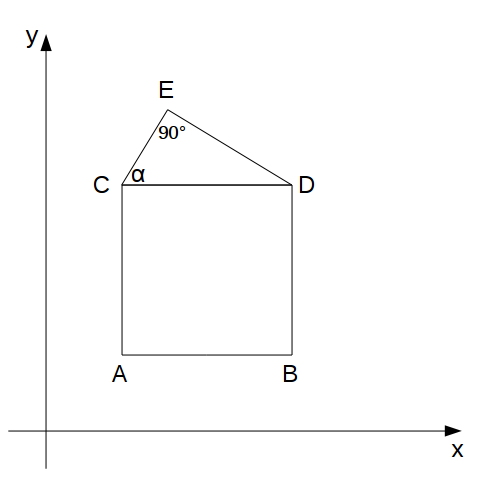
\includegraphics[width=.28\textwidth, height=.28\textwidth]{sketch.png}
\caption{Veranschaulichung der Definition}
\end{figure}
%\newline
\paragraph{Besonderheit dieser Inszenierung:}
Ein Pythagorasbaum lässt sich mit beliebigen Winkeln zeichnen, ich beschränke mich jedoch auf die drei Winkel $\alpha=30\deg,60\deg,45\deg$,
wobei $\alpha=\angle ECD$.
Im Gegensatz zu anderen Pythagorasbaumadaptionen\footnote{
\href{http://de.wikipedia.org/w/index.php?title=Datei:Pythagoras\_baum\_color\_random.png}
     {siehe z.B. http://de.wikipedia.org/w/index.php?title=Datei:Pythagoras\_baum\_color\_random.png}},
die versuchen eine möglichst realistische zweidimensionale Darstellung eines realen Baumes zu erlangen, war es hier Ziel,
eine informatisch-künstlerische Inszenierung zu erzeugen. \\
Ich verwende den Begriff Ast für ein Stamm-Quadrat, ein Dreieck und zwei Nachfolgeäste.\\
Es gibt somit drei verschiedene Äste, die ich mit folgenden Ideen implementiere:
Äste mit $\alpha=30\deg$ sollen die Sättigung verändern (nach links ungesättigter, nach rechts gesättigter) während
Äste mit $\alpha=60\deg$ den Farbton auf der Farbskala verschieben (nach links in Richtung rot, nach rechts in Richtung lila) und
Äste mit $\alpha=45\deg$ die Helligkeit manipulieren (nach links heller, rechts dunkler).
\subsection{Programm-Dokumentation}
\paragraph{Implementation:}
Es wurden eine Startregel (\emph{BAUM}), eine Hauptregel (\emph{AST}) und drei gewicht\-et\-e Teilregeln (\emph{WINKELAST}) definiert.
Jede der drei \emph{WINKELAST}-Regeln stellt jeweils einen Winkel dar und zeichnet rekursiv zwei Unteräste,
durch zweimaligem Aufruf der \emph{AST}-Regel.
Die Berechnung der Koordinaten für die Folgebäume für jeden Winkel folgt aus der Definition.
\newpage
\subsection{Programm-Ablaufprotokoll}
\subsubsection{Erzeugung}
Das verwendete Programm ``Context Free Art'' (CFDG) erzeugt Bilder durch interpetieren der Regeln,
angefangen bei einer Startregel (hier BAUM). Rekursive Regeln ohne Rekursionsschluss sind erlaubt,
das Rendern hört ab einer definierten Größe auf. Regeln lassen sich mehrdeutig definieren,
wodurch eine von diesen zufällig gezeichnet wird. Der Zufall lässt sich durch Gewichte an den Regeln beeinflussen.
Die Erzeugung des Pythagorasbaums veranschaulicht folgende Abbildung.
\begin{figure}[ht]
\centering
 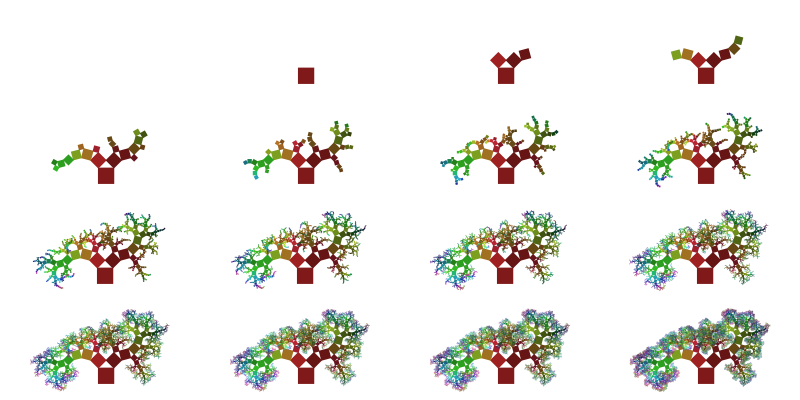
\includegraphics[width=\textwidth, height=.5\textwidth]{steps.png}
\caption{Veranschaulichung der rekursiven Erzeugung}
\end{figure}

\clearpage
\newpage
\subsubsection{Ergebnisse}
Durch veränderte Gewichte und Startfarben werden stark unterschiedliche Bäume erzeugt.
Die verschiedenen Auswirkungen erkennt man am deutlichsten,
wenn zunächst nur Bäume mit durchgehend gleichem Winkel betrachtet werden.
Dies wird für alle drei Winkel in Abbildung 1 gezeigt:
Abb. (a) zeigt das Verändern des Farbtons bei $\alpha=30\deg$.
In Abb. (b) lässt sich die Veränderung der Sättigung bei $\alpha=60\deg$ beobachten, wohingegen sich in
Abb. c die Helligkeit bei $\alpha=45\deg$ ändert.
% Grafiken für ein jeden Winkel
\begin{figure}[ht]
\centering
\subfloat[Bei $\alpha=30\deg$ verändert sich der Farbton]{
 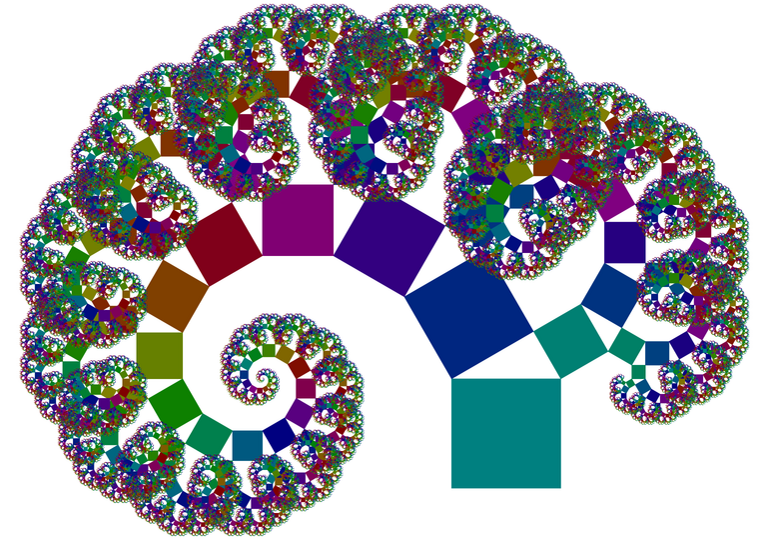
\includegraphics[width=.3\textheight, height=.2\textheight]{alpha30.png}}
\subfloat[Bei $\alpha=60\deg$ verändert sich die Sättigung]{
 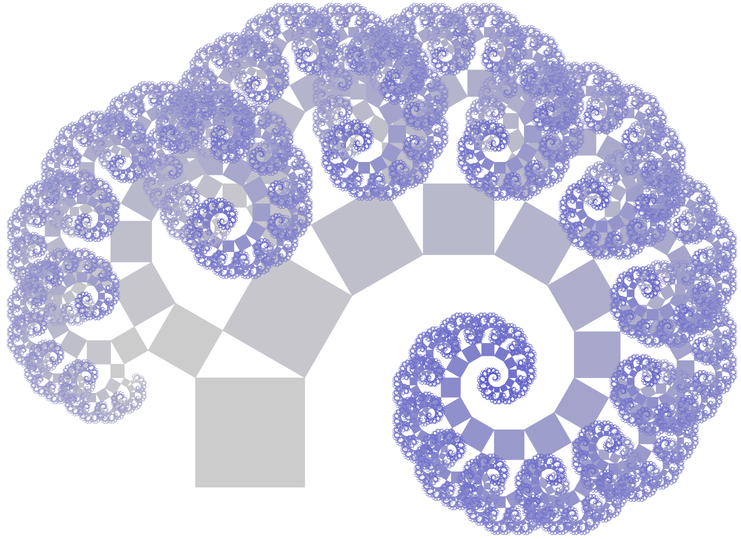
\includegraphics[width=.3\textheight, height=.2\textheight]{alpha60.png}}
\\
\subfloat[Bei $\alpha=45\deg$ verändert sich die Helligkeit]{
 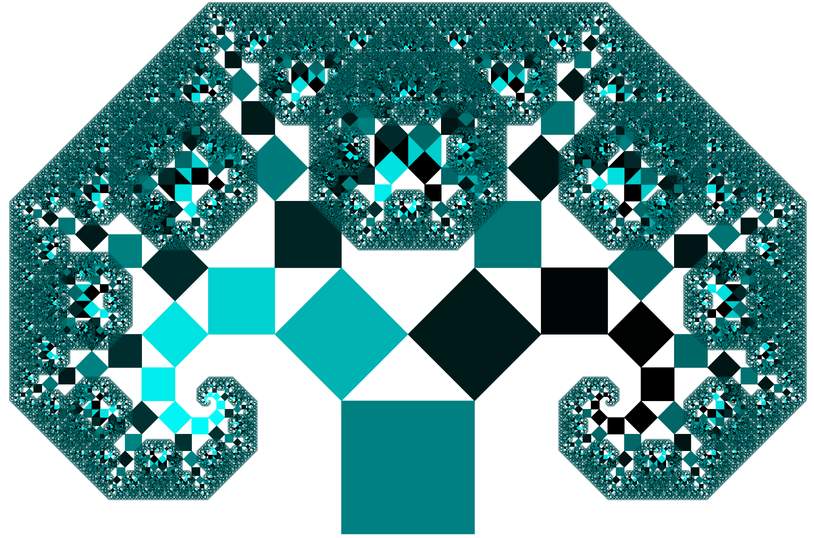
\includegraphics[width=0.92\textwidth, height=.56\textwidth]{alpha45.png}
}
\caption{Auswirkungen der verschiedenen Winkel}
\end{figure}
% Mischgrafiken (2)
\begin{figure}[ht]
 \centering
 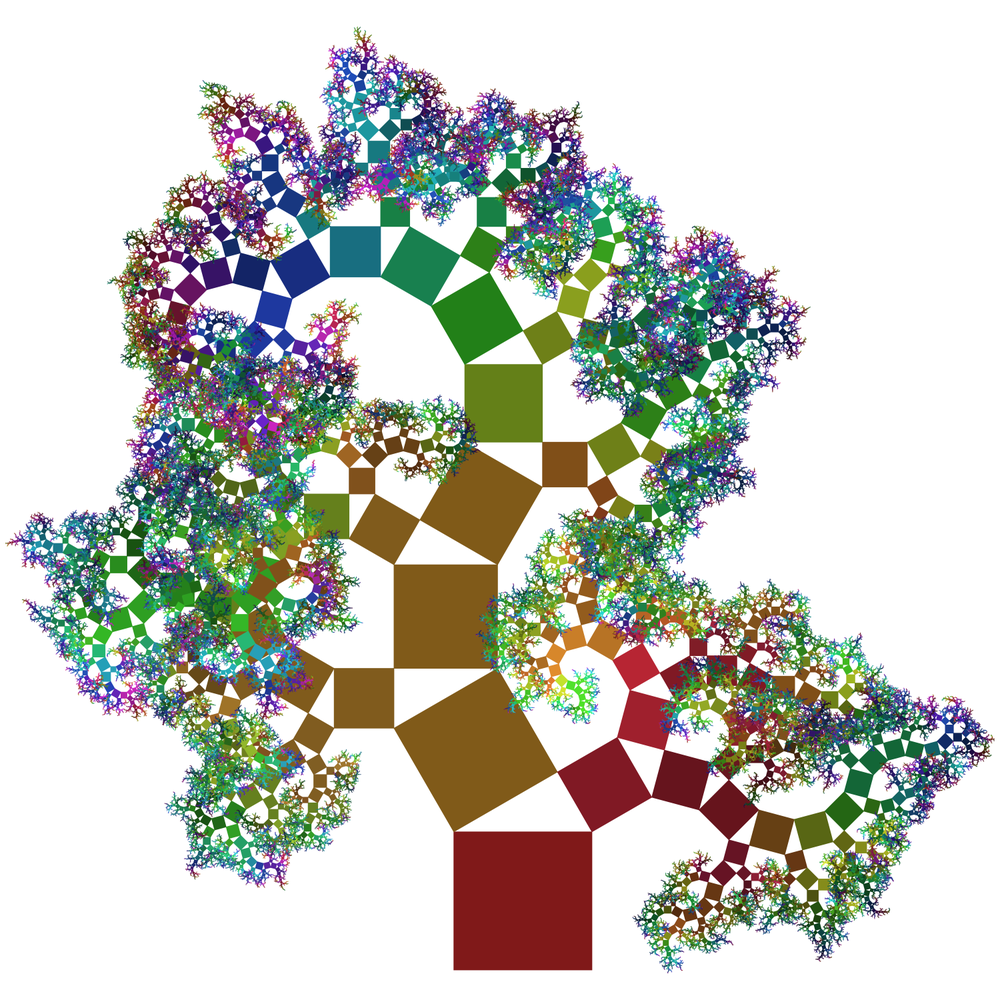
\includegraphics[width=0.72\textheight, height=0.72\textheight]{art.png}
 \caption{Ein vollständiges Kunstwerk mit Startfarbe rot}
\end{figure}
\begin{figure}[ht]
 \centering
 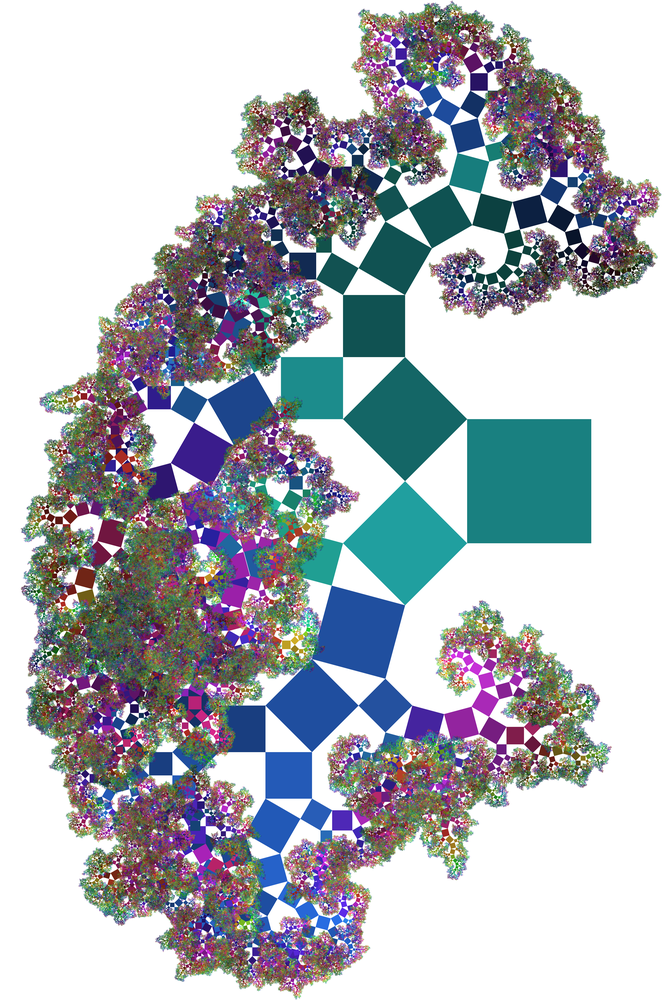
\includegraphics[width=0.666\textheight, height=\textheight]{bigrot.png}
 \caption{Ein Kunstwerk mit besonders vielen Iterationen, Startfarbe türkis}
\end{figure}
\clearpage

\subsection{Programm-Text}
Der dokumentierte Quellcode (Aufgabe1/src/baum.cfdg):
\definecolor{darkgreen}{rgb}{.03,.3117,.078}
\definecolor{darkblue}{rgb}{.03,.078,.8117}

\lstdefinelanguage{cfdg}[]{Octave}
  {morekeywords={startshape, background, rule,x,y,r,s,b,h,sat}}

\lstset{language=cfdg}
\lstset{basicstyle=\footnotesize}
\lstinputlisting{baum.cfdg}

\subsection{Programm-Nutzung}
Der Quellcode kann nicht direkt ausgeführt werden, aber er kann mit cfdg interpretiert werden.
Beachten Sie jedoch, dass jede Ausführung mit cfdg - aufgrund der durch Zufall ausgewählten Regeln - ein anderes Ergebnis erzeugt.
Die Ausführung folgt unter dem Wurzelverzeichnis mit: `cfdg Aufgabe1/src/baum.cfdg Pfad/zur/Ausgabe.png'.
Da auf die CD keine Dateien geschrieben werden können, geben Sie bitte einen Pfad an, in dem Sie die Ausgabedatei speichern möchten.
Es sind außerdem die Erzeugnisse unter `Aufgabe1/dist' enthalten.